\documentclass{homework}\usepackage[]{graphicx}\usepackage[]{color}
% maxwidth is the original width if it is less than linewidth
% otherwise use linewidth (to make sure the graphics do not exceed the margin)
\makeatletter
\def\maxwidth{ %
  \ifdim\Gin@nat@width>\linewidth
    \linewidth
  \else
    \Gin@nat@width
  \fi
}
\makeatother

\definecolor{fgcolor}{rgb}{0.345, 0.345, 0.345}
\newcommand{\hlnum}[1]{\textcolor[rgb]{0.686,0.059,0.569}{#1}}%
\newcommand{\hlstr}[1]{\textcolor[rgb]{0.192,0.494,0.8}{#1}}%
\newcommand{\hlcom}[1]{\textcolor[rgb]{0.678,0.584,0.686}{\textit{#1}}}%
\newcommand{\hlopt}[1]{\textcolor[rgb]{0,0,0}{#1}}%
\newcommand{\hlstd}[1]{\textcolor[rgb]{0.345,0.345,0.345}{#1}}%
\newcommand{\hlkwa}[1]{\textcolor[rgb]{0.161,0.373,0.58}{\textbf{#1}}}%
\newcommand{\hlkwb}[1]{\textcolor[rgb]{0.69,0.353,0.396}{#1}}%
\newcommand{\hlkwc}[1]{\textcolor[rgb]{0.333,0.667,0.333}{#1}}%
\newcommand{\hlkwd}[1]{\textcolor[rgb]{0.737,0.353,0.396}{\textbf{#1}}}%
\let\hlipl\hlkwb

\usepackage{framed}
\makeatletter
\newenvironment{kframe}{%
 \def\at@end@of@kframe{}%
 \ifinner\ifhmode%
  \def\at@end@of@kframe{\end{minipage}}%
  \begin{minipage}{\columnwidth}%
 \fi\fi%
 \def\FrameCommand##1{\hskip\@totalleftmargin \hskip-\fboxsep
 \colorbox{shadecolor}{##1}\hskip-\fboxsep
     % There is no \\@totalrightmargin, so:
     \hskip-\linewidth \hskip-\@totalleftmargin \hskip\columnwidth}%
 \MakeFramed {\advance\hsize-\width
   \@totalleftmargin\z@ \linewidth\hsize
   \@setminipage}}%
 {\par\unskip\endMakeFramed%
 \at@end@of@kframe}
\makeatother

\definecolor{shadecolor}{rgb}{.97, .97, .97}
\definecolor{messagecolor}{rgb}{0, 0, 0}
\definecolor{warningcolor}{rgb}{1, 0, 1}
\definecolor{errorcolor}{rgb}{1, 0, 0}
\newenvironment{knitrout}{}{} % an empty environment to be redefined in TeX

\usepackage{alltt}
\author{Johann Marques Viana Freitas}
\class{Econometria I: Prof. Nathalie Gimenes}
\date{\today}
\title{Lista Prática}
\address{}

\usepackage[portuguese]{babel}
\usepackage{amssymb}
\usepackage{amsmath}
\usepackage{bm}
\usepackage{tcolorbox}
\usepackage{graphicx}
\usepackage{caption}
\IfFileExists{upquote.sty}{\usepackage{upquote}}{}
\begin{document} \maketitle

\question

\section{Funções de Verossimilhança e Estimadores}

\begin{enumerate}
  \item A mistura de normais é caracterizada da seguinte forma:
  \begin{align}
    e_i \sim \begin{cases}
                \mathrm{N}(\mu_1, \sigma_1^2), \text{com probabilidade } 1/2,\\
                \mathrm{N}(\mu_2, \sigma_2^2), \text{com probabilidade } 1/2.
              \end{cases}
  \end{align}
  
  Para computar a densidade, podemos modelar $f(e_i) \sim \mathrm{Bern}(1/2)$ e calcular $\mathbb{E}_{\mathrm{Bern(1/2)}}\left[f(e_i)\right]$:
  
  \begin{align}
    \mathbb{E}_{\mathrm{Bern(1/2)}}\left[f(e_i)\right] &=
    \dfrac{1}{2}\times\left[\dfrac{1}{\sqrt{2\pi\sigma_1^2}}\mathrm{exp}\left(-\dfrac{1}{2\sigma_1^2}\left(y_i - \beta_0 - \beta_1 x_i - \mu_1 \right)^2\right) +
    \dfrac{1}{\sqrt{2\pi\sigma_2^2}}\mathrm{exp}\left(-\dfrac{1}{2\sigma_2^2}\left(y_i - \beta_0 - \beta_1 x_i - \mu_2 \right)^2\right)\right].
  \end{align}
  
  Podemos escrever a função de verossimilhança amostral como
  
  \begin{align}
    L(\bm{\beta}|\mathbf{y}, \mathbf{x}; \mu_1, \mu_2, \sigma_1^2, \sigma_2^2) &= \prod_{i=1}^n\dfrac{1}{2}\times\left[\dfrac{1}{\sqrt{2\pi\sigma_1^2}}\mathrm{exp}\left(-\dfrac{1}{2\sigma_1^2}\left(y_i - \beta_0 - \beta_1 x_i - \mu_1 \right)^2\right) +\right\\
    &\left\dfrac{1}{\sqrt{2\pi\sigma_2^2}}\mathrm{exp}\left(-\dfrac{1}{2\sigma_2^2}\left(y_i - \beta_0 - \beta_1 x_i - \mu_2 \right)^2\right)\right] \nonumber\\
    &= \dfrac{1}{2^n}\prod_{i=1}^n\times\left[\dfrac{1}{\sqrt{2\pi\sigma_1^2}}\mathrm{exp}\left(-\dfrac{1}{2\sigma_1^2}\left(y_i - \beta_0 - \beta_1 x_i - \mu_1 \right)^2\right) +\right\nonumber\\
    &\left\dfrac{1}{\sqrt{2\pi\sigma_2^2}}\mathrm{exp}\left(-\dfrac{1}{2\sigma_2^2}\left(y_i - \beta_0 - \beta_1 x_i - \mu_2 \right)^2\right)\right]. \nonumber
  \end{align}
  
  Obtendo a log-verossimilhança:
  
  \begin{align}
    l(\bm{\beta}|\mathbf{y}, \mathbf{x}; \mu_1, \mu_2, \sigma_1^2, \sigma_2^2) &= -n\mathrm{log}(2)+\sum^n_{i=1}\mathrm{log}\left(\dfrac{1}{\sqrt{2\pi\sigma_1^2}}\mathrm{exp}\left(-\dfrac{1}{2\sigma_1^2}\left(y_i - \beta_0 - \beta_1 x_i - \mu_1 \right)^2\right) +\right\\
    &\left\dfrac{1}{\sqrt{2\pi\sigma_2^2}}\mathrm{exp}\left(-\dfrac{1}{2\sigma_2^2}\left(y_i - \beta_0 - \beta_1 x_i - \mu_2 \right)^2\right)\right)\nonumber.
  \end{align}
  
  O Estimador de Máxima Verossimilhança é dado por
  
  \begin{align}
    \hat{\bm{\beta}} &= \underset{\beta_0, \beta_1}{\mathrm{argmax}}\ l(\bm{\beta}|\mathbf{y}, \mathbf{x}; \mu_1, \mu_2, \sigma_1^2, \sigma_2^2).
  \end{align}
  
  \item Função de verossimilhança amostral para $u$, com $u_i \sim \Gamma(a,b)$, definida para $u_i > 0$:
  \begin{align}
  L(\bm{\beta}|\mathbf{y}, \mathbf{x}; a, b) &= \prod_{i=1}^n{\dfrac{b^a}{\Gamma(a)}\left(y_i - \beta_1 - \beta_2 x_i\right)^{a-1}\mathrm{exp}\left(-b\left(y_i - \beta_1 - \beta_2 x_i\right)\right)}\\
  &= \left(\dfrac{b^a}{\Gamma(a)}\right)^n\prod_{i=1}^n{\left(y_i - \beta_1 - \beta_2 x_i\right)^{a-1}}\mathrm{exp}\left(-b\sum_{i=1}^n\left(y_i - \beta_1 - \beta_2 x_i\right)\right).\nonumber
  \end{align}
  
  Aplicando tranformação logarítmica
  
  \begin{align}
  l(\bm{\beta}|\mathbf{y}, \mathbf{x}; a, b) &= n\mathrm{log}\left(\dfrac{b^a}{\Gamma(a)}\right) + (a-1)\sum_{i=1}^n{\mathrm{log}\left(y_i - \beta_1 - \beta_2 x_i\right)} -b\sum_{i=1}^n\left(y_i - \beta_1 - \beta_2 x_i\right).
  \end{align}
  
  O Estimador de Máxima Verossimilhança é dado por
  
  \begin{align}
    \hat{\bm{\beta}} &= \underset{\beta_0, \beta_1}{\mathrm{argmax}}\ l(\bm{\beta}|\mathbf{y}, \mathbf{x}; a, b).
  \end{align}
  
  \item Sabemos que $v_i \sim \mathrm{Cauchy}(0,1) \sim t(\nu = 1)$, em que $\nu$ representa os graus de liberdade. Portanto, a função de verossimilhança amostral para $\mathbf{v}$, com $v_i \sim \mathrm{Cauchy}(0,1)$ pode ser escrita como:
  
  \begin{align}
    L(\bm{\beta}|\mathbf{y}, \mathbf{x}; \nu) &= \prod_{i=1}^n\dfrac{\Gamma\left(\dfrac{\nu+1}{2}\right)}{\sqrt{\nu\pi}\Gamma\left(\dfrac{\nu}{2}\right)}\left(1 + \dfrac{\left(y_i - \beta_1 - \beta_2 x_i\right)^2}{\nu}\right)\nonumber\\
    &= \left[\dfrac{\Gamma\left(\dfrac{\nu+1}{2}\right)}{\sqrt{\nu\pi}\Gamma\left(\dfrac{\nu}{2}\right)}\right]^n\prod_{i=1}^n\left(1 + \dfrac{\left(y_i - \beta_1 - \beta_2 x_i\right)^2}{\nu}\right).
  \end{align}
  
  A log-verossimilhança, por sua vez,
  
  \begin{align}
    l(\bm{\beta}|\mathbf{y}, \mathbf{x}; \nu) &= n\left[\mathrm{log}\left(\Gamma\left(\dfrac{\nu+1}{2}\right)\right)-
    \mathrm{log}\left(\sqrt{\nu\pi}\right)-
    \mathrm{log}\left(\Gamma\left(\dfrac{\nu}{2}\right)\right)\right] + \sum_{i=1}^n\mathrm{log}\left(1 + \dfrac{\left(y_i - \beta_1 - \beta_2 x_i\right)^2}{\nu}\right).
  \end{align}
  
  O Estimador de Máxima Verossimilhança é dado por
  
  \begin{align}
    \hat{\bm{\beta}} &= \underset{\beta_0, \beta_1}{\mathrm{argmax}}\ l(\bm{\beta}|\mathbf{y}, \mathbf{x}; \nu).
  \end{align}

\end{enumerate}

\section{Distribuições Assintóticas}

Vide \cite{greene2011econometric}, Teorema 14.1.M2, \textit{se são satisfeitas condições de regularidade},

\begin{align}
  \hat{\bm{\theta}} \xrightarrow{d} \mathrm{N}\left(\bm{\theta}_0, \{\mathbf{I(\bm{\theta}_0)}\}^{-1}),
\end{align}

em que $\hat{\bm{\theta}}$ é o estimador de Máxima Verossimilhança de $\bm{\theta}_0$, e $\mathbf{I(\bm{\theta}_0)} = -\mathbb{E}\left[\dfrac{\partial^2\mathrm{log}(L)}{\partial\bm{\theta}_0\partial\bm{\theta}_0^'}\right].

\renewcommand{\labelenumi}{R.\arabic{enumi}.}

\begin{tcolorbox}
{\hfill\textbf{Condições de regularidade}\hfill}

\begin{enumerate}

\item As primeiras três derivadas de $\mathrm{log}(f(y_i|\bm{\theta}))$ em relação a $\bm{\theta}$ são contínuas e finitas para quase todo $y_i$, e para todo $\bm{\theta}$.

\item As condições necessárias para obter as esperanças da primeira e da segunda derivada de $\mathrm{log}(f(y_i|\bm{\theta}))$ são satisfeitas.

\item Para todos os valores de $\bm{\theta}$, $\left|\partial^3\mathrm{log}(f(y_i|\bm{\theta}))/\partial\theta_j\partial\theta_k\partial_l\right|$ é menor que uma função com esperança finita.

\end{enumerate}

\renewcommand{\labelenumi}{\arabic{enumi}}

\end{tcolorbox}

\question

\section{Simulações}

O experimento de simulação é conduzido em \verb|R| \cite{rcore}\footnote{Soluções providas por \cite{knitr} e \cite{tidyverse} foram empregadas na análise e reporte deste exercício.}. Primeiramente, definimos parâmetros gerais para a simulação, como o tamanho da amostra e os valores verdadeiros para $\bm{\beta}$.

%\definecolor{shadecolor}{RGB}{255,255,255}



\begin{knitrout}
\definecolor{shadecolor}{rgb}{0.922, 0.922, 0.922}\color{fgcolor}\begin{kframe}
\begin{alltt}
\hlcom{# Simulating data generating processes}

\hlstd{n} \hlkwb{=} \hlnum{2000} \hlcom{# Sample size}

\hlcom{# Setting random seed}
\hlkwd{set.seed}\hlstd{(}\hlnum{1981}\hlstd{)}

\hlcom{# Exercise 2}
\hlcom{# Generating x}
\hlstd{x} \hlkwb{=} \hlkwd{rnorm}\hlstd{(}\hlkwc{n} \hlstd{= n,} \hlkwc{mean} \hlstd{=} \hlnum{5}\hlstd{,} \hlkwc{sd} \hlstd{=} \hlkwd{sqrt}\hlstd{(}\hlnum{1}\hlstd{))}

\hlcom{# Defining betas}

\hlstd{beta} \hlkwb{=} \hlkwd{c}\hlstd{(}\hlnum{2.35}\hlstd{,} \hlnum{0.75}\hlstd{)}
\end{alltt}
\end{kframe}
\end{knitrout}

Em seguida, simulamos os três processos de geração de dados. Para obter a mistura de normais, é utilizada uma variável auxiliar $P \sim \mathrm{Bernoulli}(1/2)$ e definimos $e_1 \sim \mathrm{N}(\mu_1, \sigma_1^2)$, $e_2 \sim \mathrm{N}(\mu_2, \sigma_2^2)$ e $e = Pe_1 + (1-P)e_2$.

\begin{knitrout}
\definecolor{shadecolor}{rgb}{0.922, 0.922, 0.922}\color{fgcolor}\begin{kframe}
\begin{alltt}
\hlcom{# Simulating model 1}
\hlcom{# Since \textbackslash{}mu_1, \textbackslash{}mu_2, \textbackslash{}sigma_1 and \textbackslash{}sigma_2 were not specified,}
\hlcom{# I'm considering the following}
\hlstd{mu_1} \hlkwb{=} \hlnum{2}
\hlstd{mu_2} \hlkwb{=} \hlnum{1}
\hlstd{sigma_1} \hlkwb{=} \hlkwd{sqrt}\hlstd{(}\hlnum{1.5}\hlstd{)}
\hlstd{sigma_2} \hlkwb{=} \hlkwd{sqrt}\hlstd{(}\hlnum{3}\hlstd{)}

\hlstd{e1} \hlkwb{=} \hlkwd{rnorm}\hlstd{(}\hlkwc{n} \hlstd{= n,} \hlkwc{mean} \hlstd{= mu_1,} \hlkwc{sd} \hlstd{= sigma_1)}
\hlstd{e2} \hlkwb{=} \hlkwd{rnorm}\hlstd{(}\hlkwc{n} \hlstd{= n,} \hlkwc{mean} \hlstd{= mu_2,} \hlkwc{sd} \hlstd{= sigma_2)}

\hlcom{# Defining an auxiliary random variable P ~ Bernoulli(1/2)}

\hlstd{P} \hlkwb{=} \hlkwd{rbinom}\hlstd{(}\hlkwc{n} \hlstd{= n,} \hlkwc{size} \hlstd{=} \hlnum{1}\hlstd{,} \hlkwc{prob} \hlstd{=} \hlnum{1}\hlopt{/}\hlnum{2}\hlstd{)}

\hlstd{e} \hlkwb{=} \hlstd{P} \hlopt{*} \hlstd{e1} \hlopt{+} \hlstd{(}\hlnum{1}\hlopt{-}\hlstd{P)} \hlopt{*} \hlstd{e2}

\hlstd{y_1} \hlkwb{=} \hlstd{beta[}\hlnum{1}\hlstd{]} \hlopt{+} \hlstd{beta[}\hlnum{2}\hlstd{]} \hlopt{*} \hlstd{x} \hlopt{+} \hlstd{e}
\end{alltt}
\end{kframe}
\end{knitrout}

\begin{knitrout}
\definecolor{shadecolor}{rgb}{0.922, 0.922, 0.922}\color{fgcolor}\begin{kframe}
\begin{alltt}
\hlkwd{tibble}\hlstd{(e1, e2)} \hlopt
  \hlkwd{pivot_longer}\hlstd{(}\hlkwc{cols} \hlstd{=} \hlkwd{c}\hlstd{(}\hlstr{'e1'}\hlstd{,} \hlstr{'e2'}\hlstd{))} \hlopt
  \hlkwd{ggplot}\hlstd{(}\hlkwd{aes}\hlstd{(}\hlkwc{x} \hlstd{= value,} \hlkwc{group} \hlstd{= name))} \hlopt{+}
    \hlkwd{geom_histogram}\hlstd{(}\hlkwd{aes}\hlstd{(}\hlkwc{y} \hlstd{=} \hlkwd{after_stat}\hlstd{(density),} \hlkwc{fill} \hlstd{= name),}
                   \hlkwc{alpha} \hlstd{=} \hlnum{.8}\hlstd{,} \hlkwc{position} \hlstd{=} \hlstr{'identity'}\hlstd{,} \hlkwc{binwidth} \hlstd{=} \hlnum{0.25}\hlstd{,} \hlkwc{color} \hlstd{=} \hlstr{'black'}\hlstd{)} \hlopt{+}
  \hlkwd{labs}\hlstd{(}\hlkwc{fill} \hlstd{=} \hlstr{''}\hlstd{,} \hlkwc{x} \hlstd{=} \hlstr{''}\hlstd{,} \hlkwc{y} \hlstd{=} \hlstr{''}\hlstd{)} \hlopt{+} \hlkwd{scale_fill_manual}\hlstd{(}\hlkwc{values} \hlstd{= purple_rain_colors[}\hlkwd{c}\hlstd{(}\hlnum{1}\hlstd{,}\hlnum{2}\hlstd{)])}

\hlkwd{ggplot}\hlstd{()} \hlopt{+}
  \hlkwd{geom_histogram}\hlstd{(}\hlkwd{aes}\hlstd{(}\hlkwc{y} \hlstd{=} \hlkwd{after_stat}\hlstd{(density),} \hlkwc{x} \hlstd{= e),}
                 \hlkwc{alpha} \hlstd{=} \hlnum{.8}\hlstd{,} \hlkwc{position} \hlstd{=} \hlstr{'identity'}\hlstd{,} \hlkwc{binwidth} \hlstd{=} \hlnum{0.25}\hlstd{,} \hlkwc{color} \hlstd{=} \hlstr{'black'}\hlstd{,}
                 \hlkwc{fill} \hlstd{= purple_rain_colors[}\hlnum{3}\hlstd{])} \hlopt{+}
  \hlkwd{labs}\hlstd{(}\hlkwc{fill} \hlstd{=} \hlstr{''}\hlstd{,} \hlkwc{x} \hlstd{=} \hlstr{''}\hlstd{,} \hlkwc{y} \hlstd{=} \hlstr{''}\hlstd{)}
\end{alltt}
\end{kframe}\begin{figure}
\subfloat[$e_1$ e $e_2$\label{fig:Simul1-1}]{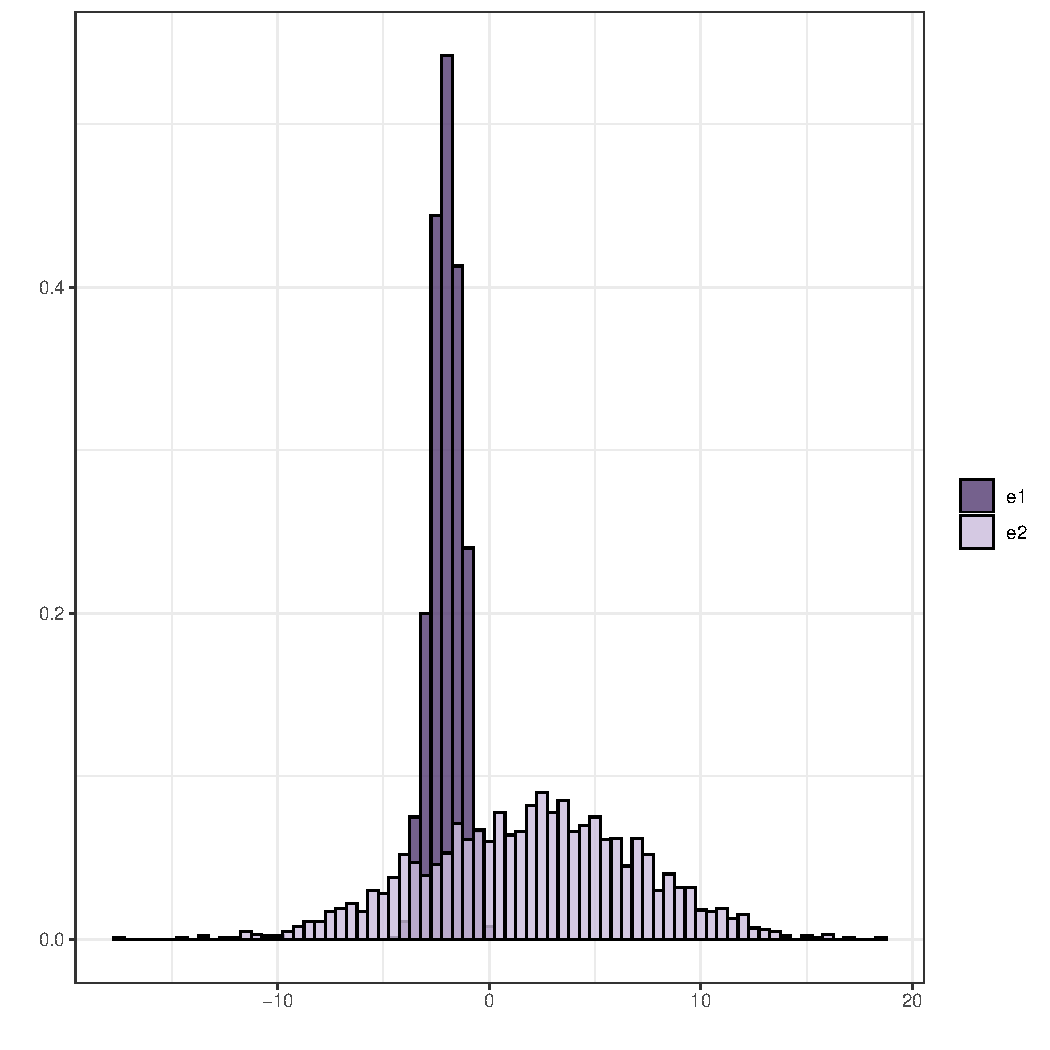
\includegraphics[width=.49\linewidth]{figure/Simul1-1} }
\subfloat[Mistura\label{fig:Simul1-2}]{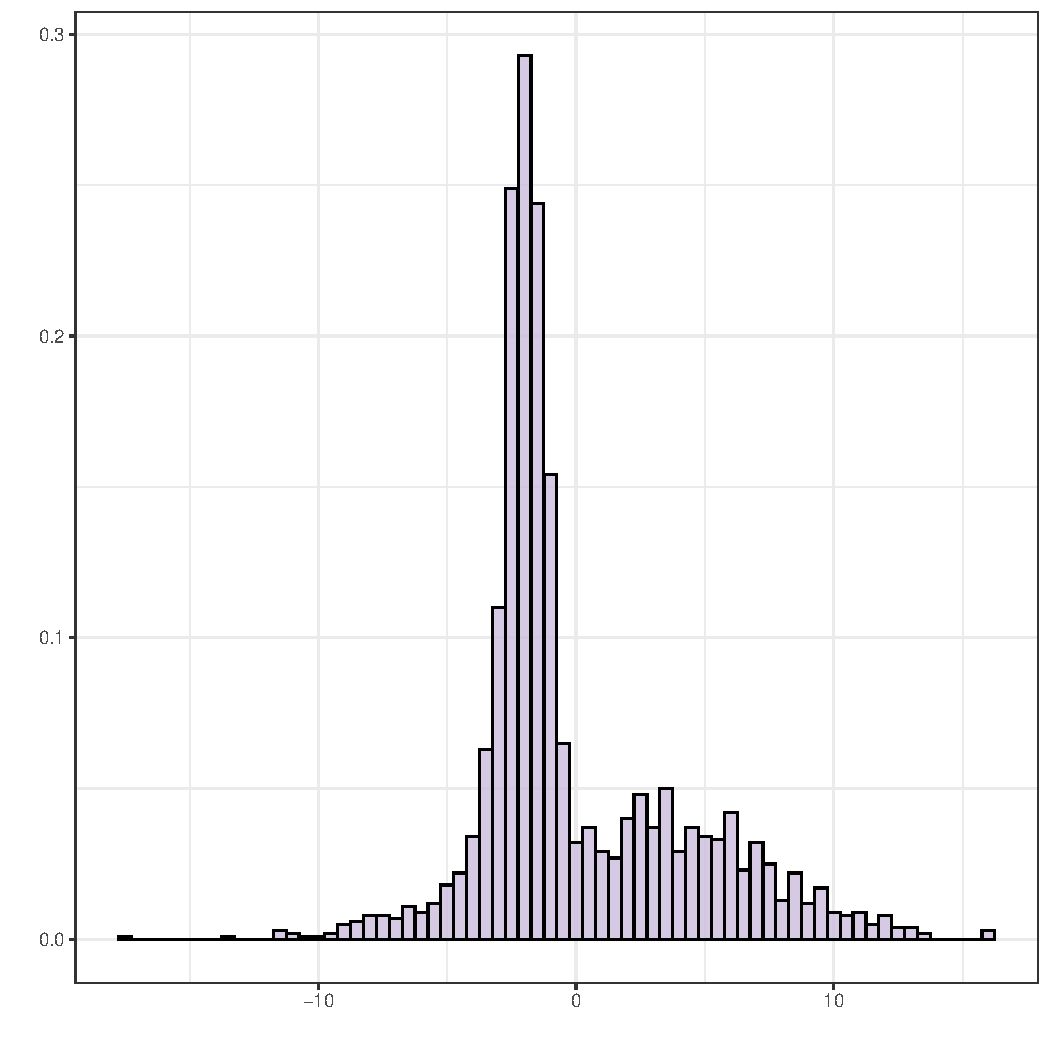
\includegraphics[width=.49\linewidth]{figure/Simul1-2} }\caption[Distribuições de $e_1$, $e_2$, $e$]{Distribuições de $e_1$, $e_2$, $e$}\label{fig:Simul1}
\end{figure}

\end{knitrout}

\begin{knitrout}
\definecolor{shadecolor}{rgb}{0.922, 0.922, 0.922}\color{fgcolor}\begin{kframe}
\begin{alltt}
\hlcom{# Simulating model 2}
\hlcom{# Since a and b were not specified, I'm considering the following}

\hlstd{a} \hlkwb{=} \hlnum{1.75}
\hlstd{b} \hlkwb{=} \hlnum{.8}

\hlstd{u} \hlkwb{=} \hlkwd{rgamma}\hlstd{(}\hlkwc{n} \hlstd{= n,} \hlkwc{shape} \hlstd{= a,} \hlkwc{rate} \hlstd{= b)}

\hlstd{y_2} \hlkwb{=} \hlstd{beta[}\hlnum{1}\hlstd{]} \hlopt{+} \hlstd{beta[}\hlnum{2}\hlstd{]} \hlopt{*} \hlstd{x} \hlopt{+} \hlstd{u}
\end{alltt}
\end{kframe}
\end{knitrout}

\begin{knitrout}
\definecolor{shadecolor}{rgb}{0.922, 0.922, 0.922}\color{fgcolor}\begin{kframe}
\begin{alltt}
\hlcom{# Simulating model 3}

\hlstd{v} \hlkwb{=} \hlkwd{rt}\hlstd{(}\hlkwc{n} \hlstd{= n,} \hlkwc{df} \hlstd{=} \hlnum{1}\hlstd{)}

\hlstd{y_3} \hlkwb{=} \hlstd{beta[}\hlnum{1}\hlstd{]} \hlopt{+} \hlstd{beta[}\hlnum{2}\hlstd{]} \hlopt{*} \hlstd{x} \hlopt{+} \hlstd{v}
\end{alltt}
\end{kframe}
\end{knitrout}

\section{Estatísticas descritivas}

\begin{kframe}
\begin{alltt}
\hlkwd{print}\hlstd{(}\hlkwd{xtable}\hlstd{(}\hlkwd{map_df}\hlstd{(}\hlkwd{list}\hlstd{(x, e1, e2, y_1, u, y_2, v, y_3),} \hlopt{~}\hlkwd{summary}\hlstd{(.x))} \hlopt
               \hlstd{\{}\hlkwd{cbind}\hlstd{(}\hlkwd{data.frame}\hlstd{(}\hlstr{'Variable'} \hlstd{=} \hlkwd{c}\hlstd{(}\hlstr{"$\textbackslash{}\textbackslash{}bar\{x\}$"}\hlstd{,} \hlstr{"$\textbackslash{}\textbackslash{}bar\{e\}_1$"}\hlstd{,}
                                                \hlstr{"$\textbackslash{}\textbackslash{}bar\{e\}_2$"}\hlstd{,} \hlstr{"$\textbackslash{}\textbackslash{}bar\{y\}_1$"}\hlstd{,}
                                                \hlstr{"$\textbackslash{}\textbackslash{}bar\{u\}$"}\hlstd{,} \hlstr{"$\textbackslash{}\textbackslash{}bar\{y\}_2$"}\hlstd{,}
                                                \hlstr{"$\textbackslash{}\textbackslash{}bar\{v\}$"}\hlstd{,} \hlstr{"$\textbackslash{}\textbackslash{}bar\{y\}_3$"}\hlstd{)),}
                      \hlstd{.)\},}
             \hlstd{,}
      \hlkwc{caption} \hlstd{=} \hlstr{'Estatísticas descritivas'}\hlstd{),}
      \hlkwc{sanitize.text.function}\hlstd{=}\hlkwa{function}\hlstd{(}\hlkwc{x}\hlstd{)\{x\},} \hlkwc{include.rownames} \hlstd{=} \hlnum{FALSE}\hlstd{)}
\end{alltt}
\end{kframe}% latex table generated in R 4.1.2 by xtable 1.8-4 package
% Sun May 14 20:38:18 2023
\begin{table}[ht]
\centering
\begin{tabular}{lrrrrrr}
  \hline
Variable & Min. & 1st Qu. & Median & Mean & 3rd Qu. & Max. \\ 
  \hline
$\bar{x}$ & 1.81 & 4.27 & 4.97 & 4.98 & 5.69 & 8.46 \\ 
  $\bar{e}_1$ & -1.95 & 1.19 & 2.00 & 2.01 & 2.87 & 5.88 \\ 
  $\bar{e}_2$ & -5.83 & -0.19 & 1.07 & 0.99 & 2.18 & 6.76 \\ 
  $\bar{y}_1$ & 1.19 & 6.41 & 7.63 & 7.56 & 8.76 & 12.92 \\ 
  $\bar{u}$ & 0.03 & 0.99 & 1.76 & 2.18 & 2.94 & 13.91 \\ 
  $\bar{y}_2$ & 4.68 & 7.00 & 7.96 & 8.27 & 9.18 & 21.09 \\ 
  $\bar{v}$ & -2163.94 & -1.01 & -0.01 & 1.48 & 0.98 & 5489.95 \\ 
  $\bar{y}_3$ & -2158.61 & 4.84 & 6.05 & 7.57 & 7.33 & 5495.47 \\ 
   \hline
\end{tabular}
\caption{Estatísticas descritivas} 
\end{table}


% citations
\bibliographystyle{plain}
\bibliography{citations}

\end{document}
